\section{Quotientenräume}

Seien $V,W$ $K$-Vektorräume und $U\subseteq V$ ein Untervektorraum.

\begin{definition}[affiner Unterraum]
	Ein \begriff{affiner Unterraum} von $V$ ist eine Teilmenge der Form 
	\begin{align}
		x+U:=\{x+u\mid u \in U\}\subseteq V\notag
	\end{align}
	wobei $U\subseteq V$ ein beliebiger Untervektorraum von $V$ ist und $x\in V$.
\end{definition}

\begin{definition}[Quotientenraum]
	Der \begriff{Quotientenraum} von $V$ modulo $U$ ist die Menge der affinen Unterräume
	\begin{align}
		\qraum{V}{U}:=\{x+U\mid x\in V\}\notag
	\end{align}
	mit der Addition $(x_1+U)+(x_2+U)=(x_1+x_2)+U$ und der Multiplikation $\lambda(x+U)=\lambda x+U$. Dies ist 
	wohldefiniert nach \propref{3_7_5}.
	
	Wir definieren die Abbildung $\pi_U:V\to$ \qraum{$V$}{$U$} durch $\pi_U(x)=x+U$.
\end{definition}

\begin{remark}
	Die Untervektorraum sind also genau die Kerne linearer Abbildungen! Ist $f:V\to W$ linear, so ist $\Ker(f)\subseteq V$ ein Untervektorraum. 
	Ist $U\subseteq V$ ein Untervektorraum, so ist $\pi_U:V\to$\qraum{$V$}{$U$} linear mit Kern $U$.
\end{remark}

\begin{theorem}[Homomorphiesatz]
	\proplbl{3_7_9}
	Sei $f\in \Hom_K(V,W)$ mit $U\subseteq \Ker(f)$. Dann gibt es genau eine lineare Abbildung $\tilde f:$
	\qraum{$V$}{$U$}$\to W$ mit $f=\tilde f \circ \pi_U$, d.h. es kommutiert: \\
	\begin{center}
		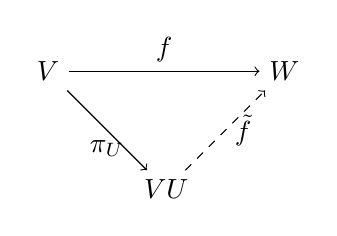
\begin{tikzpicture}
		\node (V) at (0,0) {$V$};
		\node (W) at (3,0) {$W$};
		\node (R) at (1.5,-1.5) {\qraum{$V$}{$U$}};
		\draw[->, above] (V) to node {$f$} (W);
		\draw[->, below] (V)  to node {$\pi_U$} (R);
		\draw[->, right, dashed] (R)  to node {$\tilde f$} (W);
		\end{tikzpicture}
	\end{center}
	Diese erfüllt $\Ker(\tilde f)=$\qraum{$\Ker(f)$}{U}$=\{x+U\mid x\in \Ker(f)\}\subseteq$\qraum{$V$}{$U$}.
\end{theorem}
\begin{proof}
	Ist $f=\tilde f\circ \pi_U$, so gilt $\tilde f(x+U)=\tilde f(\pi_U)=f(x)\; (*)$, somit ist $\tilde f$ dann eindeutig bestimmt. Umgekehrt 
	wird durch $(*)$ eine wohldefinierte Abbildung $\tilde f$ erklärt: Sind $x,x'\in V$ mit $x+U=x'+U$, so ist $x-x'\in U\subseteq \Ker(f)$ und 
	deshalb $f(x)=f(x')$. \\
	\begin{itemize}
		\item Linearität: Für $x,y\in V$ und $\lambda\in K$ ist $\tilde f(\lambda(x+U)+\mu(y+U))=\tilde f(\lambda\pi_U(x)+\mu\pi_U(y))=\lambda\tilde f
		(x+U)+\mu\tilde f(y+U)$.
		\item Kern: $\tilde f(x+U)=0\iff f(x)=0 \iff x\in \Ker(f)$.
	\end{itemize}
\end{proof}